\documentclass[a4paper,12pt]{article}

\usepackage[utf8]{inputenc}
\usepackage[T2A]{fontenc}
\usepackage[english,russian]{babel}
\usepackage{titling}
\usepackage[flushmargin]{footmisc}
\usepackage{lipsum}
\usepackage[raggedright]{titlesec}
\usepackage{hyperref}
\usepackage{hyphenat}
\usepackage[centering]{geometry}
\usepackage{setspace}
\usepackage[table]{xcolor}

\usepackage{graphicx}
\graphicspath{{./figs/}}
\usepackage{tikz}
\usepackage{epstopdf}
\usepackage{floatrow}
%table caption on top
\usepackage{float}
\floatstyle{plaintop}
\restylefloat{table}
%%%
\usepackage{amsthm,amsfonts,amsmath,amssymb,amscd,bm}
\usepackage{listings}
\usepackage{multirow}

\newcommand\preprint[1]{\renewcommand\thepreprint{#1}}
\newcommand\thepreprint{\@latex@error{No \noexpand\preprint given}\@ehc}

\newcommand\institute[1]{\renewcommand\theinstitute{#1}}
\newcommand\theinstitute{\@latex@error{No \noexpand\institute given}\@ehc}

\renewcommand\abstract[1]{\renewcommand\theabstract{#1}}
\newcommand\theabstract{\@latex@error{No \noexpand\abstract given}\@ehc}

\newcommand\preparedfor[1]{\renewcommand\thepreparedfor{#1}}
\newcommand\thepreparedfor{\@latex@error{No \noexpand\preparedfor given}\@ehc}

\newcommand\keywords[1]{\renewcommand\thekeywords{#1}}
\newcommand\thekeywords{\@latex@error{No \noexpand\keywords given}\@ehc}

\newcommand\acknowledgements[1]{\renewcommand\theacknowledgements{#1}}
\newcommand\theacknowledgements{\@latex@error{No \noexpand\acknowledgements given}\@ehc}

\newtheorem{theorem}{Теорема}[section]

\newcommand\thepreprints{Препринты}
\newcommand\thepreprintsurl{Все препринты доступны на сайте \url{http://chpc.ru/preprints}.}

\newcommand\blfootnote[1]{
  \begingroup
  \renewcommand\thefootnote{}\footnote{#1}
  \addtocounter{footnote}{-1}
  \endgroup
}

\renewcommand\maketitle{
\begin{titlepage}
	\begin{center}
		\begin{footnotesize}
			
\includegraphics[width=0.1\linewidth]{nefu.png}

			\vspace{3mm}			

			Северо-Восточный федеральный университет им. М.К. Аммосова \\
			Научно-исследовательская кафедра вычислительных технологий
		\end{footnotesize}
	\end{center}		
	
	\vfill
	
	\begin{center}
		\begin{LARGE}
			\fontsize{20pt}{32pt}\textbf{\thetitle}\par
		\end{LARGE}

		\vspace{10mm}

		\theauthor

		\vspace{10mm}

		Препринт \thepreprint
	\end{center}

	\vfill
	
	\begin{center}
		\begin{footnotesize}
			
\includegraphics[width=0.08\linewidth]{logo.png}
			
			\vspace{3mm}

			г. Якутск 
			
			\the\year
		\end{footnotesize}
	\end{center}

\end{titlepage}

	\thispagestyle{empty}
	
	\null
	
	\vfill

	\noindent\thepreparedfor
	
	\cleardoublepage

	\setcounter{page}{1}

	\begin{center}
		\begin{Large}
			\textbf{\thetitle}
		\end{Large}
	
		\vspace{5mm}
	
		\theauthor
		\blfootnote{\theinstitute}

		\vspace{5mm}

		\textbf{Аннотация} 
	\end{center}

	\theabstract

	\vspace{5mm}

	\textbf{Ключевые слова:} \thekeywords
		
	\vspace{5mm}

	%\textbf{Благодарности} \theacknowledgements	
}
% организация листингов
\usepackage{color}
\definecolor{gr}{rgb}{0.97,.97,0.97}
\definecolor{gr1}{rgb}{0.9,.9,0.9}
\definecolor{gr2}{rgb}{0.9,.5,0.}

\usepackage{listings}
\lstloadlanguages{[ANSI]C,[ANSI]C++}
\lstset{
	language=[ANSI]{C},
	keywordstyle=\bfseries\ttfamily\color[rgb]{0,0,1},
	identifierstyle=\ttfamily,
	commentstyle=\color[rgb]{0.133,0.545,0.133},
	stringstyle=\ttfamily\color[rgb]{0.627,0.126,0.941},
	showstringspaces=false,
	basicstyle=\small,
	numberstyle=\footnotesize,
	tabsize=4,
	breaklines=true,
	prebreak = \raisebox{0ex}[0ex][0ex]{\ensuremath{\hookleftarrow}},
	breakatwhitespace=false,
	aboveskip={1.5\baselineskip},
  	columns=fixed,
  	upquote=true,
  	extendedchars=true,
 	frame=single,
	backgroundcolor=\color{gr},
	rulecolor=\color{gr1}
}
\renewcommand{\lstlistingname}{Листинг}
 
\usepackage{tikz}
\usepackage{pgfplots}
\usetikzlibrary{er}
\usetikzlibrary{shapes,arrows}

\begin{document}
\newcolumntype{L}[1]{>{\raggedright\arraybackslash}p{#1}}
\newcolumntype{C}[1]{>{\centering\arraybackslash}p{#1}}
\newcolumntype{R}[1]{>{\raggedleft\arraybackslash}p{#1}}

\section{Постановка задачи}
Моделируется нестационарный процесс в ядерном реакторе в транспортном SP$_3$ приближении \cite{brantley2000}. Динамика нейтронного потока рассматривается в ограниченной выпуклой двухмерной или трехмерной области  $\Omega$ ($\bm x = \{x_1, ..., x_d\} \in \Omega, \ d = 2,3$) с границей $\partial \Omega$. 
Перенос нейтронов описывается системой уравнений:
\begin{equation}\label{1.1}
\begin{split}
 \frac{1}{v_g} \frac{\partial \phi_{0,g}}{\partial t} - \frac{2}{v_g} \frac{\partial \phi_{2,g}}{\partial t} - & \nabla \cdot D_{0,g} \nabla \phi_{0,g} + \Sigma_{r,g} \phi_{0,g} -  2\Sigma_{r,g} \phi_{2,g} = \\ 
 =  & (1-\beta)\chi_{n,g} S_{n,g} + S_{s,g} + \chi_{d,g} S_d, \\
 \frac{9}{v_g} \frac{\partial \phi_{2,g}}{\partial t} - \frac{2}{v_g} \frac{\partial \phi_{0,g}}{\partial t} - & \nabla \cdot D_{2,g} \nabla \phi_{2,g} + (5\Sigma_{t,g} + 4\Sigma_{r,g}) \phi_{2,g} -  2\Sigma_{r,g} \phi_{0,g} = \\ 
 =  & -2(1-\beta)\chi_{n,g} S_{n,g} - 2S_{s,g} - 2\chi_{d,g} S_d,
\end{split}
\end{equation}
% \ (1-\beta) \chi_g \sum_{g'=1}^{G} \nu \Sigma_{fg'} \phi_{g'} + \widetilde{\chi}_g \sum_{m=1}^{M} \lambda_m c_m 
% - \sum_{g\neq g'=1}^{G} \Sigma_{s,g'\rightarrow g} \phi_{g'} 
где
\[
S_{n,g} =  \sum_{g'=1}^{G} \nu \Sigma_{f,g'} \phi_{g'}, 
\quad
S_{s,g} = \sum_{g\neq g'=1}^{G} \Sigma_{s,g'\rightarrow g} \phi_{g'},
\quad
S_{d} = \sum_{m=1}^{M} \lambda_m c_m,
\]
\[
\phi_{0,g}=\phi_g + 2\phi_{2,g}, 
\quad
D_{0,g} = \cfrac{1}{3\Sigma_{tr,g}}, 
\quad
D_{2,g} = \cfrac{9}{7\Sigma_{t,g}}, 
\quad g=1,2,...,G.
\]
Здесь $G$ --- число групп,
$\phi_g(\bm x)$ --- скалярный поток нейтронов,
$\phi_{0,g}(\bm x)$ --- псевдо 0-й момент углового потока,
$\phi_{2,g}(\bm x)$ --- второй момент углового потока ,
$\Sigma_{t,g}$ --- полное сечение, 
$\Sigma_{tr,g}$ --- транспортное сечение, 
 $\Sigma_{r,g}(\bm x)$ --- сечение увода,
$\Sigma_{s,g'\rightarrow g}(\bm x)$ --- сечение рассеяния,
$\chi_g$  --- спектр нейтронов, 
$\nu\Sigma_{f,g}(\bm x)$ --- сечение генерации,
$c_m$ --- плотность источников запаздывающих нейтронов,
$\lambda_m$ --- постоянная распада источников запаздывающих нейтронов,
$M$ --- число типов запаздывающих нейтронов.

Плотность источников запаздывающих нейтронов описывается уравнениями
\begin{equation}\label{1.2}
 \frac{\partial c_m}{\partial t} + \lambda_m c_m = \beta_m \sum_{g=1}^{G} \nu \Sigma_{f,g} \phi_g,
 \quad m = 1,2, ..., M, 
\end{equation}
где $\beta_m$ --- доля запаздывающих нейтронов  $m$ типа, причем
\[
 \beta = \sum_{m=1}^{M} \beta_m.
\] 
На границе области $\partial \Omega$ ставятся граничные условия Маршака:
\begin{equation}\label{1.3}
\begin{split}
\begin{bmatrix}
J_{0,g}(\bm x)\\
J_{2,g}(\bm x)\\
\end{bmatrix}
=
\begin{bmatrix}
\phantom{-}\cfrac{1}{2} & -\cfrac{3}{8} \\
 -\cfrac{3}{8} & \phantom{-}\cfrac{21}{8} \\
\end{bmatrix}
\begin{bmatrix}
\phi_{0,g}(\bm x) \\
\phi_{2,g}(\bm x) \\
\end{bmatrix},
\quad
J_{i,g}(\bm x) = -D_{i,g}\nabla\phi_{i,g}(\bm x), 
\quad
i = 0, 2.
\end{split}
\end{equation}

Рассматривается задача для системы уравнений (\ref{1.1}), (\ref{1.2}) с краевыми условиями (\ref{1.3}), и начальными условиями:
\begin{equation}\label{1.4}
 \phi_g(\bm x,0) = \phi_g^0(\bm x), 
  \quad  g = 1,2, ..., G ,
 \quad   c_m(\bm x,0) = c_m^0(\bm x), 
  \quad  m = 1,2, ..., M.
\end{equation}

\subsection{Операторная формулировка}
Запишем краевую задачу (\ref{1.1})--(\ref{1.4}) в операторной форме. 
Определим векторы решений $\bm u = \{u_1, u_2, \cdots, u_G\}$, $u_g = \{\phi_{0,g}, \phi_{2,g}\}$, $\bm c = \{c_1, c_2, ..., c_M\}$ и матрицы
\[
V = (\mathrm{v}_{gg'}),
\quad
\mathrm{v}_{gg'} =\delta_{gg'} \begin{bmatrix}
\cfrac{1}{v_g} & -\cfrac{2}{v_g} \\
-\cfrac{2}{v_g} & \cfrac{9}{v_g} \\
\end{bmatrix},
\quad
D = (d_{gg'}),
\quad
d_{gg'} = \delta_{gg'} \begin{bmatrix}
D_{0,g} & 0 \\
0 & D_{2,g} \\
\end{bmatrix},
\]
\[
A = (a_{gg'}),
\quad
a_{gg} = \begin{bmatrix}
\Sigma_{r,g} &  -2\Sigma_{r,g} \\
-2\Sigma_{r,g} & 5\Sigma_{t,g} + 4\Sigma_{r,g} \\
\end{bmatrix},
\quad
a_{gg'} = \begin{bmatrix}
-\Sigma_{s, g'\rightarrow g} & 2\Sigma_{s, g'\rightarrow g} \\
2\Sigma_{s, g'\rightarrow g} & -4\Sigma_{s, g'\rightarrow g} \\
\end{bmatrix},
\]
\[
F = (f_{gg'}),
\quad
f_{gg'} = \begin{bmatrix}
\chi_{n,g}\nu\Sigma_{f,g'} & -2\chi_{n,g}\nu\Sigma_{f,g'} \\
-2\chi_{n,g}\nu\Sigma_{f,g'} & 4\chi_{n,g}\nu\Sigma_{f,g'} \\
\end{bmatrix},
\quad
B =(b_{gm}),
\quad
b_{gm} = \begin{bmatrix}
\chi_{d,g}\lambda_m\\
-2\chi_{d,g}\lambda_m\\
\end{bmatrix},
\]
\[
\Lambda = (\lambda_{mm'}), 
\quad
\lambda_{mm'} = \delta_{mm'}\lambda_m,
\quad
Q = (q_{mg})
\quad
q_{mg} =\beta_m \begin{bmatrix}
\nu\Sigma_{f,g} \\
-2\nu\Sigma_{f,g} \\
\end{bmatrix},
\]
где
\[
 \delta_{g g'} = \left \{ 
 \begin{matrix}
 1, & g = g', \\
 0, & g \neq  g',
 \end{matrix}
 \right. 
\] 
есть символ Кронеккера.
Будем работать на множестве векторов $\bm u$, компоненты которого удовлетворяют граничным условиям (\ref{1.3}).
С учетом введенных обозначений система уравнений (\ref{1.1}), (\ref{1.2}) записывается в следующем виде:
\begin{equation}\label{1.5}
\begin{split}
V \frac{d \bm{u}}{d t} -\nabla \cdot D \nabla \bm u  + A \bm{u} &=(1-\beta) F \bm{u} + B\bm c,
\\
\frac{d \bm c}{d t} + \Lambda \bm c &= Q \bm{u}. 
\end{split}
\end{equation}
Без учета запаздывающих нейтронов имеем
\begin{equation}\label{1.6}
V \frac{d \bm{u}}{d t} -\nabla \cdot D \nabla \bm{u}  + A \bm{u} = F \bm{u}.
\end{equation}  
Для (\ref{1.5}) и (\ref{1.6}) рассматривается задача Коши, когда
\begin{equation}\label{1.7}
 \bm u(0) = \bm u^0, \quad \bm c(0) = \bm c^0,
\end{equation} 
где $\bm u^0 = \{u^0,  u_2^0, ...,  u_G^0 \}$ и 
$\bm c^0 = \{ c_1^0,  c_2^0, ...,  c_M^0 \}$.

\subsection{$\lambda$-спектральная задача}
Для характеристики динамических процессов в ядерном реакторе, которые описываются задачей Коши (\ref{1.5})-(\ref{1.7}), применяются решения некоторых спектральных задач \cite{Bell1970,hetrick1971dynamics,stacey2007}.
Обычно рассматривается спектральная задача, которая известна как $\lambda$-спектральная задача.
Для системы уравнений (\ref{1.6}), (\ref{1.7}) без учета запаздывающих нейтронов, имеем
\begin{equation}\label{1.8}
-\nabla \cdot D \nabla \bm \varphi + A  \bm \varphi  = \lambda^{(k)} F \bm \varphi.
\end{equation}
Для характеристики нейтронного поля привлекается минимальное собственное значение, так что
\[
 k = \frac{1}{\lambda^{(k)}_1}  
\] 
есть эффективный коэффициент размножения.
Значение $k = \lambda^{(k)}_1 = 1$ связано с критическим состоянием реактора, а соответствующая собственная функция $\bm{\varphi}^{(1)}(\bm x)$ есть стационарное решение уравнения (\ref{1.5}), (\ref{1.6}).
При $k > 1$  говорят о надкритическом состоянии реактора, при $k < 1$  --- о подкритическом состоянии.

%В силу несамосопряженности операторов нейтронного переноса будем иметь, вообще говоря, комплексные собственные значения.
%Свойство действительности и положительности для системы уравнений нейтроники  доказывается на основе принципа максимума при некоторых ограничениях на коэффициенты операторов переноса нейтронов\cite{habetler1961existence}.
%Это касается также и несамосопряженного эллиптического оператора второго порядка\cite{bookEvans}.

\section{Численные примеры}

\subsection{Тест TWIGL 2D}
Рассматривается двухмерный транспортный тест \cite{twigl} для SP$_3$ метода. 
Моделирутся 1/4 часть активной зоны, размеры которой составляют 160x160 см.
На рисунке \ref{ris:twigl} показана геометрическая модель активной зоны, где цифрами показаны кассеты различных сортов.  
Нейтронно-физические константы теста представлены в таблице \ref{table:coeff}. 
Среднегрупповые скорости нейтронов в тесте одинаковы для всей среды и составляют $v_1 = 10^7$ см/с и $v_2 = 2 \cdot 10^5$ см/с. 
Спектр деления для мгновенных и запаздывающих нейтронов также одинаков для всей среды и равен $\chi_1 = 1$ и $\chi_2 = 0$.
В тесте представлена одна эффективная группа запаздывающих нейтронов. 
Эффективная доля запаздывающих нейтронов составляет $\beta = 0.0075$, а постоянная распада предшественников запаздывающих нейтронов $\lambda = 0.08$ с$^{-1}$.  

\begin{figure}[ht]
\begin{center}
	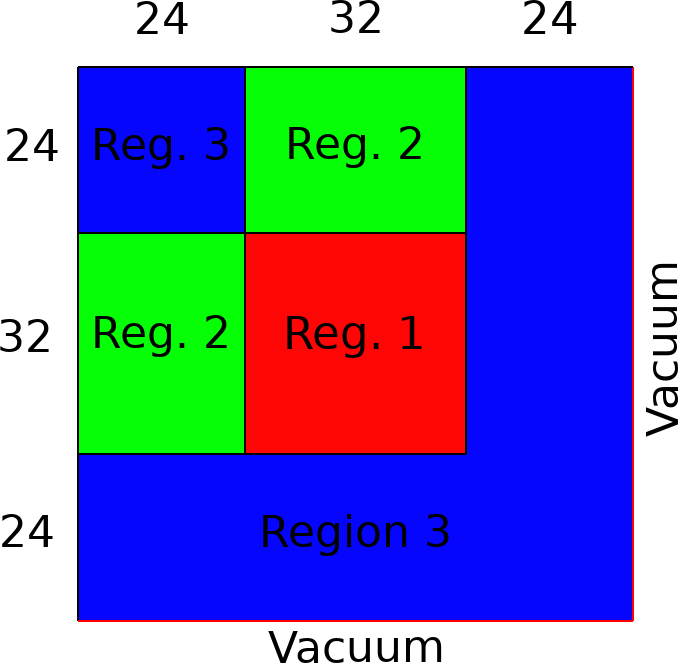
\includegraphics[width=0.6\linewidth]{twigl.png}\\
	\caption{\label{image:canonsummary}Геометрическая модель 1/4 активной зоны теста TWIGL-2D.}
	\label{ris:twigl}
\end{center}
\end{figure}

\begin{table}[htp]
\caption{\label{table:coeff}Диффузионные константы для теста TWIGL-2D.}
\label{t1}
\begin{center}
\begin{tabular}{rrrr}
\hline
Материал & 1 & 2 & 3\\
\hline 
$\Sigma_{t1}$ & 0.2481 & 0.2481 & 0.2644 \\
$\Sigma_{t2}$ & 0.9833 & 0.9833 & 0.7167 \\
$\Sigma_{a1}$ & 0.01 & 0.01 & 0.008\\
$\Sigma_{a2}$ & 0.15 & 0.15 & 0.05\\
$\Sigma_{s,1\rightarrow2}$ & 0.01 & 0.01  & 0.01\\
$\Sigma_{s,1\rightarrow1}$ & 0.2281 & 0.2281 & 0.2464\\
$\Sigma_{s,2\rightarrow2}$ & 0.8333 & 0.8333 & 0.6667\\
$\nu_1\Sigma_{f1}$ & 0.007 & 0.007 & 0.003\\
$\nu_2\Sigma_{f2}$ & 0.2 & 0.2 & 0.06\\
\hline
\end{tabular}
\end{center}
\end{table}

В задаче представлены три сценария развития переходного процесса: возмущение скачком TWIGL-S, линейное возмущение TWIGL-R и комбинированное TWIGL-C. Все возмущения происходят в зоне 1.
Возмущение скачком инициируется посредством уменьшения теплового сечения деления $\Sigma_{a2}$ на $0.0035$ см$^{-1}$ в нулевой момент времени. 
В случае линейного возмущения $\Sigma_{a2}$ линейно уменьшается на $0.0035$ см$^{-1}$ в течение $0.2$ секунд.
Комбинированное возмущение происходит следующим образом:
$\Sigma_{a2}$ линейно уменьшается на $0.0035$ см$^{-1}$ в течении $0.2$ секунд; в момент времени $0.2$ секунд происходит скачкообразное увеличение на $0.00525$ см$^{-1}$; линейно увеличивается на $0.00175$ см$^{-1}$  с момента времени $0.2$ секунд до $0.4$ секунд;  скачкообразное уменьшение на $0.0035$ см$^{-1}$.
В комбинированном случае представлены другие параметры для запаздывающих нейтронов: $v_1 = 10^7$ см/с и $v_2 = 10^5$ см/с; эффективная доля запаздывающих нейтронов составляет $\beta = 0.0064$;  постоянная распада предшественников запаздывающих нейтронов $\lambda = 0.08$ с$^{-1}$. 
Динамическое поведение исследуется на интервале $0 \leq t \leq 0.5$ с для всех трех случаев. 

\subsection{Решение $\lambda$-спектральной задачи}
Результаты расчета теста TWIGL-2D приведены в таблице \ref{table:t2-lamda}.
Здесь приняты следующие обозначения: 
$n$ --- число расчетных ячеек (конечных элементов) на кассету 24x24 в плане; 
$p$ --- порядок конечных элементов;
$k_{dif}$ --- эффективный коэффициент размножения по диффузионной модели; $k_{sp_3}$ --- эффективный коэффициент размножения по транспортной SP$_3$ модели. 
На рисунках \ref{ris:dif_pwr_0.5}, \ref{ris:dif_pwr_100}, \ref{ris:sp3_pwr} показаны расчеты нормированных мощностей для трех случаев. 

\begin{table}[h]
\caption{Результаты расчета $\lambda$-спектральной задачи.}
\label{table:t2-lamda}
\begin{center}
\begin{tabular}{r r R{2.5cm} R{2.5cm} R{2.5cm}}
\hline
$n$ & $p$ & $k_{dif} (\gamma=0.5)$ & $k_{dif} (\gamma=100)$ & $k_{sp_3}$\\
\hline
	& 1	& 0.915519 & 0.913286 & 0.916144\\
9	& 2	& 0.915519 & 0.913333 & 0.916190\\
	& 3	& 0.915419 & 0.913234 & 0.916094\\ 
\hline
	& 1	& 0.915486 & 0.913288 & 0.916147\\
36& 2	& 0.915423 & 0.913238 & 0.916096\\
	& 3	& 0.915408 & 0.913223 & 0.916076\\ 
\hline
	& 1	& 0.915434 & 0.913245 & 0.916102\\
144& 2	& 0.915409 & 0.913223 & 0.916076\\
	& 3	& 0.915408 & 0.913222 & 0.916073\\
\hline
\end{tabular}
\end{center}
\end{table}

\begin{figure}[htp]
\begin{center}
	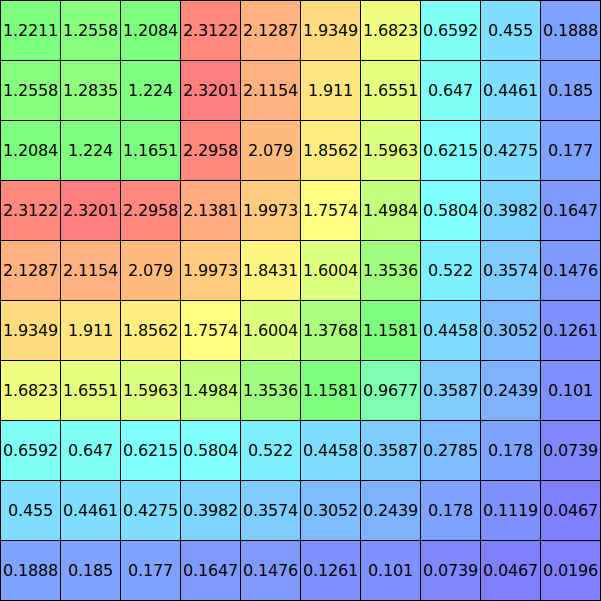
\includegraphics[width=0.65\linewidth]{dif_pwr.png}\\
	\caption{\label{image:canonsummary} Нормированная мощность по диффузионной модели при $\gamma=0.5$.}
	\label{ris:dif_pwr_0.5}
\end{center}
\end{figure}

\begin{figure}[htp]
\begin{center}
	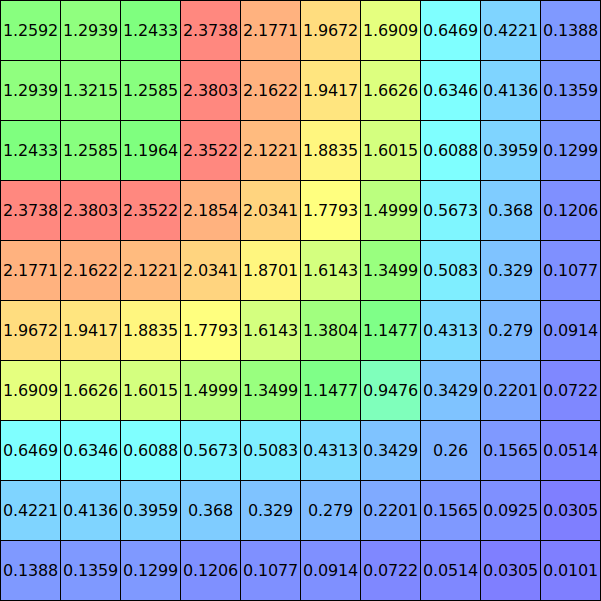
\includegraphics[width=0.65\linewidth]{dif_pwr_100.png}\\
	\caption{\label{image:canonsummary} Нормированная мощность по диффузионной модели при $\gamma=100$.}
	\label{ris:dif_pwr_100}
\end{center}
\end{figure}

\begin{figure}[htp]
\begin{center}
	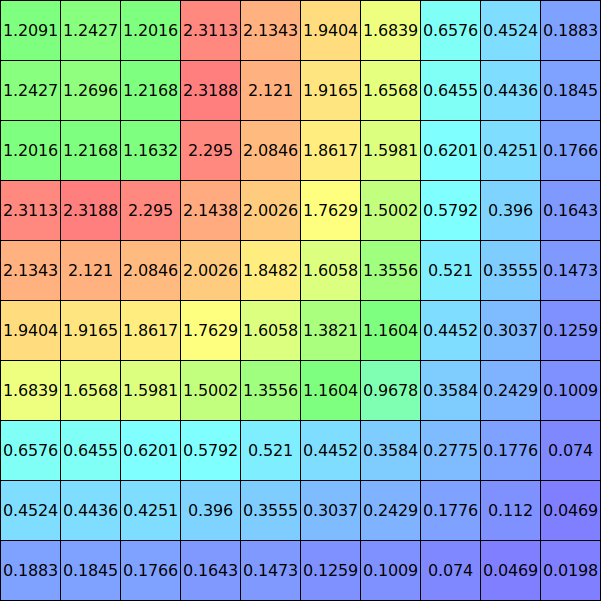
\includegraphics[width=0.65\linewidth]{sp3_pwr.png}\\
	\caption{\label{image:canonsummary} Нормированная мощность по транспортной модели.}
	\label{ris:sp3_pwr}
\end{center}
\end{figure}

\subsection{Решение $\alpha$-спектральной задачи}
В качестве «эталонного» решения взято решения полученное по модели (диффузионной или транспортной) на мелкой сетке $p=3, n=96$. 
Здесь приняты следующие обозначения: $\alpha_{dif}$ --- $\alpha$ собственное значение по диффузионной модели; $\alpha_{sp_3}$ --- $\alpha$-собственное значение по SP$_3$ модели; $\Delta$ --- абсолютное отклонение от «эталонного» значения. 

\textbf{Без учета запаздывающих нейтронов.}

В таблице~\ref{table:t2-alpha} показаны результаты расчета $\alpha$-спектральной задачи без учета запаздывающих нейтронов при использовании различных сеток и конечных элементов.
В таблице~\ref{table:t3-without} приведены результаты первых десяти собственных значений $\alpha$-спектральной задачи без учета запаздывающих нейтронов при мелкой сетке $p=3, n=96$. 
На рисунках \ref{ris:eigen1_without}, \ref{ris:eigen2_without}, \ref{ris:eigen3_without} показаны собственные функции для SP$_3$ модели.
 
\begin{table}[htp]
\caption{Результаты расчета $\alpha$-спектральной задачи.}
\label{table:t2-alpha}
\begin{center}
\begin{tabular}{r r R{2cm} R{2cm} R{2cm}}
\hline
$n$ & $p$ & $\alpha_{dif}$ $(\gamma=0.5)$ & $\alpha_{dif}$ $(\gamma=100)$ & $\alpha_{sp_3}$\\
\hline
	& 1	& 1086.39 & 1118.17 & 1082.17\\
9	& 2	& 1075.48 & 1106.20 & 1070.66\\
	& 3	& 1074.73 & 1105.38 & 1069.67\\ 
\hline
	& 1	& 1077.93 & 1108.89 & 1073.20\\
36& 2	& 1074.77 & 1105.42 & 1069.69\\
	& 3	& 1074.66 & 1105.31 & 1069.51\\ 
\hline
	& 1	& 1075.52 & 1106.25 & 1070.51\\
144& 2	& 1074.66 & 1105.31 & 1069.51\\
	& 3	& 1074.65 & 1105.30 & 1069.49\\
\hline
\end{tabular}
\end{center}
\end{table}

\begin{table}[htp]
\caption{\label{tab:canonsummary}Первые десять собственных значений $\alpha_i=\lambda_i^{(\alpha)}$ при $p=3, n=96$.}
\label{table:t3-without}
\begin{center}
\begin{tabular}{c r r r}
\hline
$i$ & Dif ($\gamma=0.5$) & Dif ($\gamma=100$) & SP$_3$ \\
\hline
1 & 1074.65 + 0.0$i$& 1105.30 + 0.0$i$ & 1069.49 + 0.0$i$ \\
2 & 2372.88 + 0.0$i$& 2471.91 + 0.0$i$ & 2350.57 + 0.0$i$ \\
3 & 2627.51 + 0.0$i$& 2773.17 + 0.0$i$ & 2597.47 + 0.0$i$ \\
4 & 3175.23 + 0.0$i$& 3326.51 + 0.0$i$ & 3131.63 + 0.0$i$ \\
5 & 3957.45 + 0.0$i$& 4106.06 + 0.0$i$ & 3889.73 + 0.0$i$ \\
6 & 4192.97 + 0.0$i$& 4291.70 + 0.0$i$ & 4119.26 + 0.0$i$ \\
7 & 4362.12 + 0.0$i$& 4481.13 + 0.0$i$ & 4281.96 + 0.0$i$ \\
8 & 4742.27 + 0.0$i$& 4777.35 + 0.0$i$ & 4649.39 + 0.0$i$ \\
9 & 5050.62 + 0.0$i$& 5180.50 + 0.0$i$ & 4944.38 + 0.0$i$ \\
10& 5309.81 + 0.0$i$& 5455.79 + 0.0$i$ & 5192.20 + 0.0$i$ \\
\hline
\end{tabular}
\end{center}
\end{table}

\begin{figure}[htp]
\begin{center}
	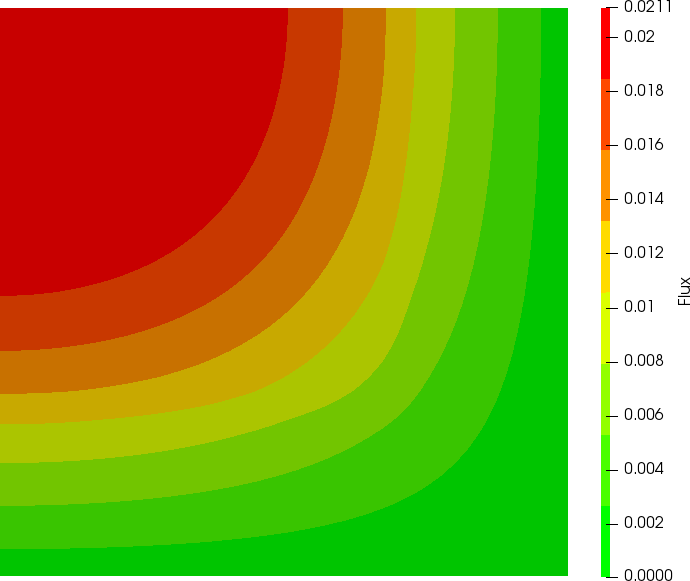
\includegraphics[width=0.49\linewidth]{sp3_alpha_u1_1.png}
	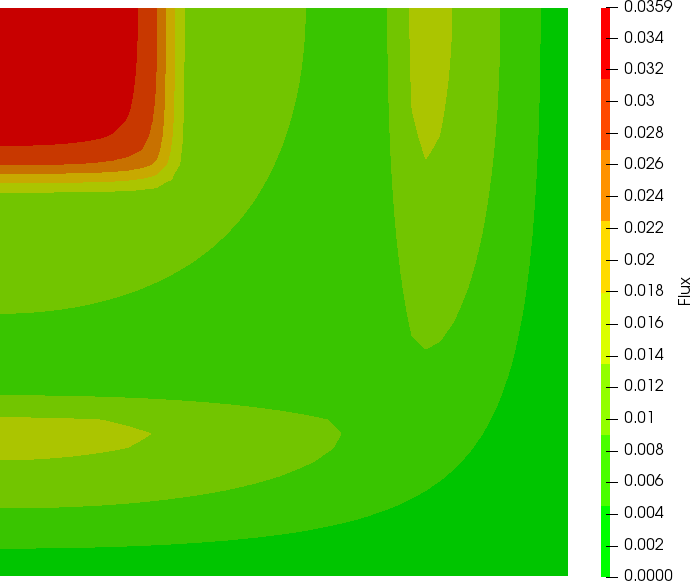
\includegraphics[width=0.49\linewidth]{sp3_alpha_u2_1.png}\\
	\caption{\label{image:canonsummary}Собственные функции $\phi_1^{(1)}$, $\phi_2^{(1)}$.}
	\label{ris:eigen1_without}
\end{center}
\end{figure}

\begin{figure}[htp]
\begin{center}
	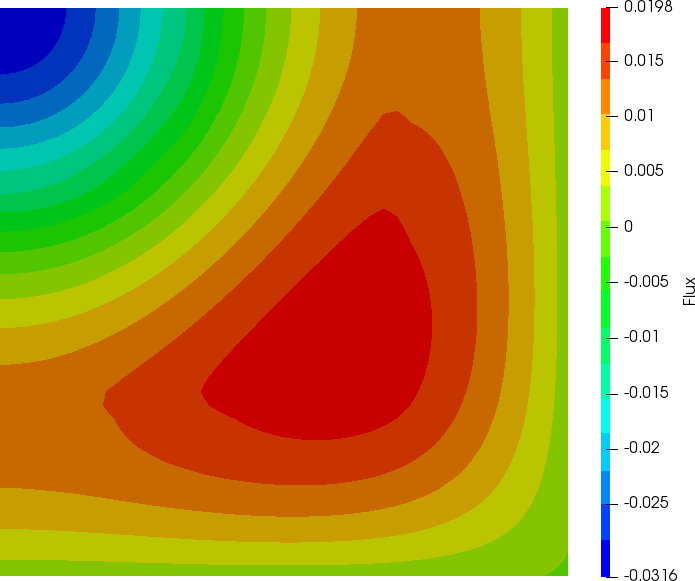
\includegraphics[width=0.49\linewidth]{sp3_alpha_u1_2.png}
	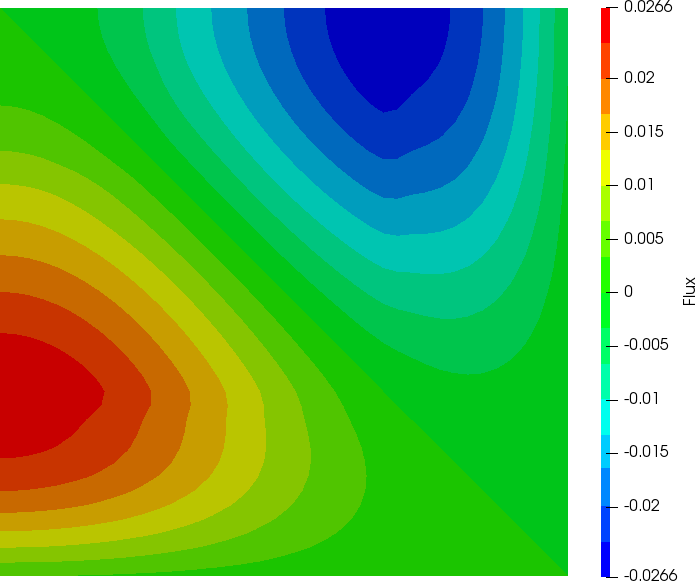
\includegraphics[width=0.49\linewidth]{sp3_alpha_u1_3.png}\\
	\caption{\label{image:canonsummary}Собственные функции $\phi_1^{(2)}$, $\phi_1^{(3)}$.}
	\label{ris:eigen2_without}
\end{center}
\end{figure}

\begin{figure}[htp]
\begin{center}
	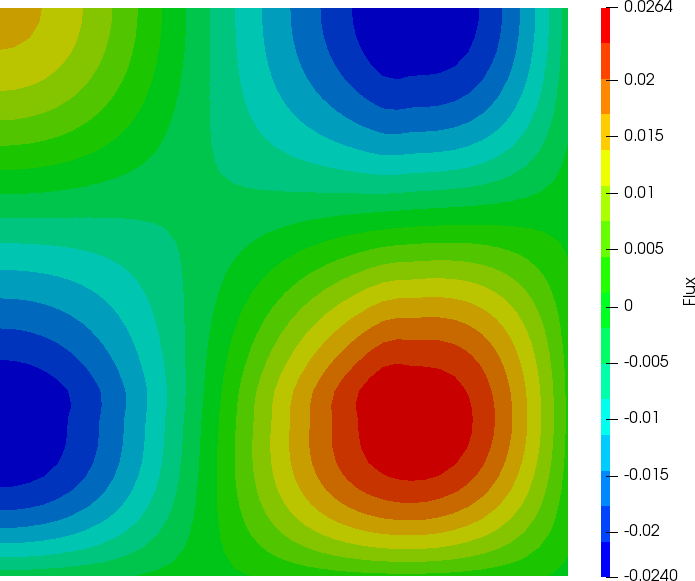
\includegraphics[width=0.49\linewidth]{sp3_alpha_u1_4.png}
	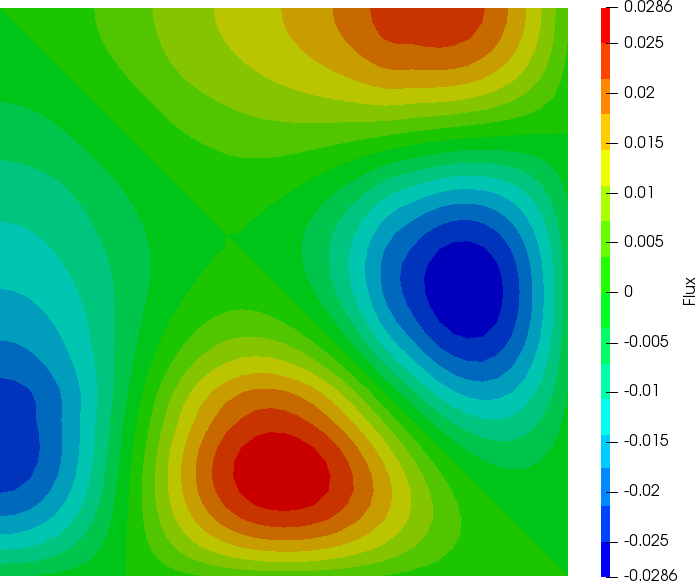
\includegraphics[width=0.49\linewidth]{sp3_alpha_u1_5.png}\\
	\caption{\label{image:canonsummary}Собственные функции $\phi_1^{(4)}$, $\phi_1^{(5)}$.}
	\label{ris:eigen3_without}
\end{center}
\end{figure}
\pagebreak
\newpage
\subsection{Решение нестационарной задачи}
Представлены исследования различных шагов по времени для всех трех сценариев.  В качестве сетки по пространству взят вариант при $n=36,\ p=2$, а для эталонного решения взяты результаты на мелкой сетке $n=144,\ p=3,\ \tau=1$ мс.

\subsubsection{Сценарий №1}
В таблице \ref{table:twigl-s} представлены результаты эталонных решений TWIGL-S при $n=144, p=3, \tau=1$ мс по диффузионной и транспортной моделях.
На рисунке \ref{ris:sp3_ref_s} показано эталонное решение TWIGL-S по транспортной модели, а на рисунке \ref{ris:odds_s} показаны различия диффузионных эталонных решений относительно транспортного эталонного решения. 
Далее, на рисунках \ref{ris:dif_tau_s_0.5}, \ref{ris:dif_tau_s_100}, \ref{ris:sp3_tau_s} показаны отличия при различных шагах по времени относительно эталонных решений.

\begin{table}[htp]
\caption{Различие результатов диффузионного и транспортного расчетов для TWIGL-S.}
\label{table:twigl-s}
\begin{center}
\begin{tabular}{r R{2.5cm} R{2.5cm} R{2.5cm}}
\hline
$t$ & Dif ($\gamma=0.5$) & Dif ($\gamma=100$) & SP$_3$\\
\hline
0.0 & 1.0000 & 1.0000 & 1.0000\\
0.1 & 2.0783  & 2.0613 & 2.0898\\
0.2 & 2.0961 & 2.0786 & 2.1079\\
0.3 & 2.1139 & 2.0959 & 2.1260\\
0.4 & 2.1319 & 2.1135 & 2.1442\\
0.5 & 2.1500 & 2.1311 & 2.1626\\
\hline
\end{tabular}
\end{center}
\end{table}

\begin{figure}[htp]
\begin{center}
	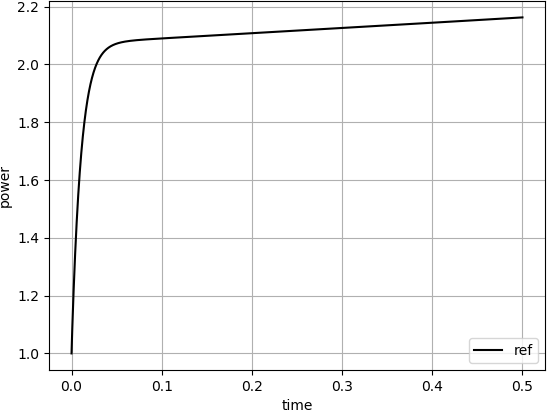
\includegraphics[width=0.8\linewidth]{sp3_ref_s.png}\\
	\caption{\label{image:canonsummary} Эталонное решение TWIGL-S по транспортной SP$_3$ модели.}
	\label{ris:sp3_ref_s}
\end{center}
\end{figure}

\begin{figure}[htp]
\begin{center}
	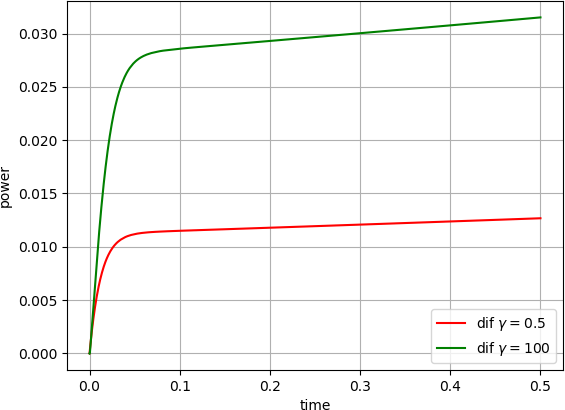
\includegraphics[width=0.8\linewidth]{odds_s.png}\\
	\caption{\label{image:canonsummary} Различия решения TWIGL-S по диффузионной модели от транспортной модели.}
	\label{ris:odds_s}
\end{center}
\end{figure}

\begin{figure}[htp]
\begin{center}
	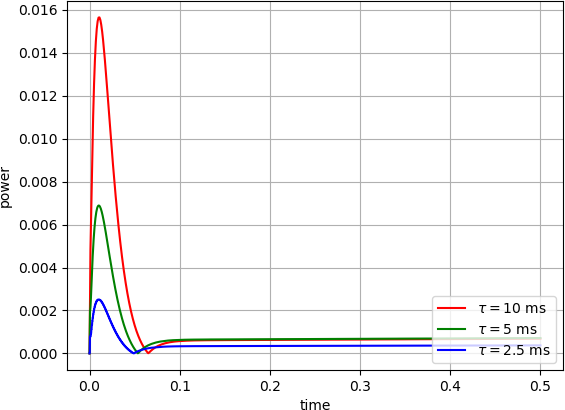
\includegraphics[width=0.8\linewidth]{dif_tau_s.png}\\
	\caption{\label{image:canonsummary} Результаты расчета TWIGL-S для различных шагов по времени по диффузионной модели при $\gamma=0.5$.}
	\label{ris:dif_tau_s_0.5}
\end{center}
\end{figure}

\begin{figure}[htp]
\begin{center}
	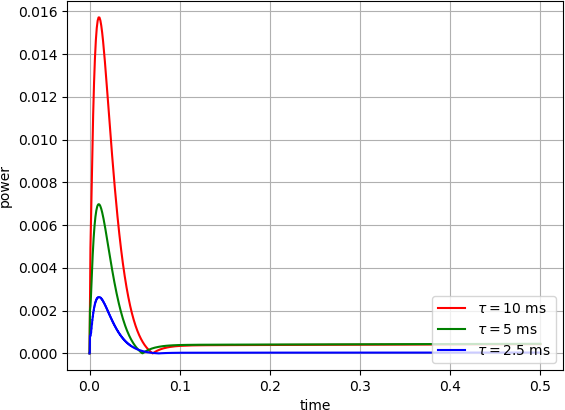
\includegraphics[width=0.8\linewidth]{dif_tau_s_100.png}\\
	\caption{\label{image:canonsummary} Результаты расчета TWIGL-S для различных шагов по времени по диффузионной модели при $\gamma=100$.}
	\label{ris:dif_tau_s_100}
\end{center}
\end{figure}

\begin{figure}[htp]
\begin{center}
	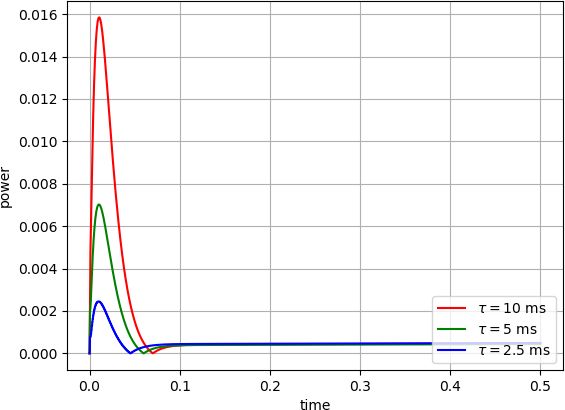
\includegraphics[width=0.8\linewidth]{sp3_tau_s.png}\\
	\caption{\label{image:canonsummary} Результаты расчета TWIGL-S для различных шагов по времени по транспортной sp3 модели.}
	\label{ris:sp3_tau_s}
\end{center}
\end{figure}

\pagebreak
\newpage

\subsubsection{Cценарий №2}
В таблице \ref{table:twigl-r} представлены результаты эталонных решений TWIGL-R при $n=144, p=3, \tau=1$ мс по диффузионной и транспортной моделях.
На рисунке \ref{ris:sp3_ref_r} показано эталонное решение TWIGL-R по транспортной модели, а на рисунке \ref{ris:odds_r} показаны различия диффузионных эталонных решений относительно транспортного эталонного решения. 
Далее, на рисунках \ref{ris:dif_tau_r_0.5}, \ref{ris:dif_tau_r_100}, \ref{ris:sp3_tau_r} показаны отличия при различных шагах по времени относительно эталонных решений.

\begin{table}[htp]
\caption{Различие результатов диффузионного и транспортного расчетов для TWIGL-R.}
\label{table:twigl-r}
\begin{center}
\begin{tabular}{r R{2.5cm} R{2.5cm} R{2.5cm}}
\hline
$t$ & Dif ($\gamma=0.5$) & Dif ($\gamma=100$) & SP$_3$\\
\hline
0.0 & 1.0000 & 1.0000 & 1.0000\\
0.1 & 1.3112  & 1.3083 & 1.3134\\
0.2 & 1.9729 & 1.9595 & 1.9826\\
0.3 & 2.0921 & 2.0747 & 2.1038\\
0.4 & 2.1099 & 2.0921 & 2.1219\\
0.5 & 2.1278 & 2.1096 & 2.1401\\
\hline
\end{tabular}
\end{center}
\end{table}

\begin{figure}[htp]
\begin{center}
	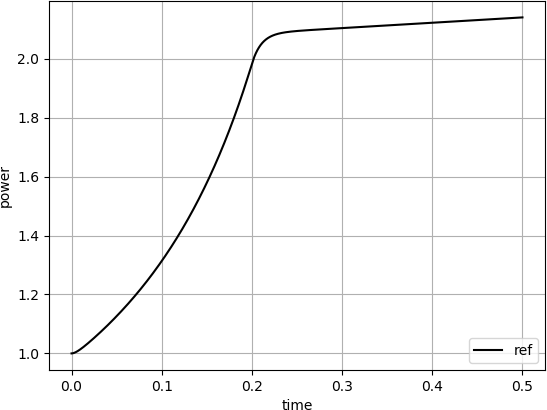
\includegraphics[width=0.8\linewidth]{sp3_ref_r.png}\\
	\caption{\label{image:canonsummary} Эталонное решение TWIGL-R по транспортной SP$_3$ модели.}
	\label{ris:sp3_ref_r}
\end{center}
\end{figure}

\begin{figure}[htp]
\begin{center}
	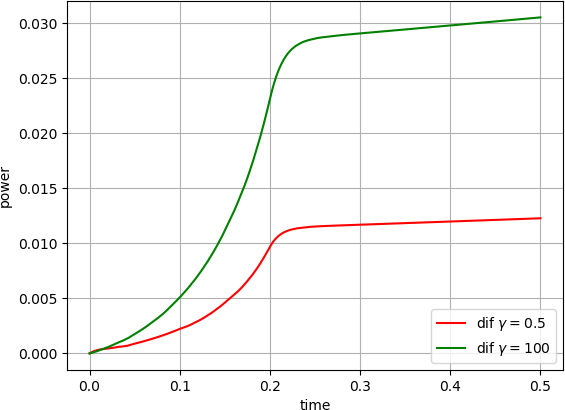
\includegraphics[width=0.8\linewidth]{odds_r.png}\\
	\caption{\label{image:canonsummary} Различия решения TWIGL-R по диффузионной модели от транспортной модели.}
	\label{ris:odds_r}
\end{center}
\end{figure}

\begin{figure}[htp]
\begin{center}
	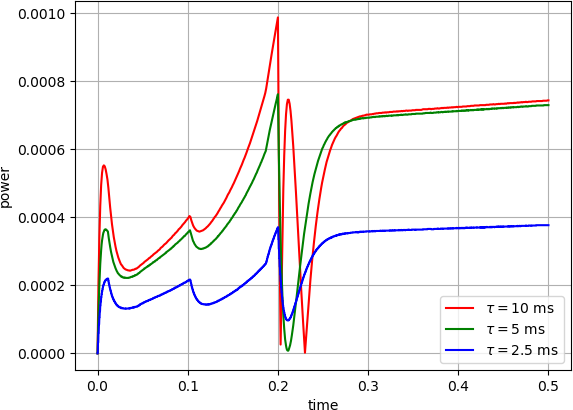
\includegraphics[width=0.8\linewidth]{dif_tau_r.png}\\
	\caption{\label{image:canonsummary}Результаты расчета TWIGL-R для различных шагов по времени по диффузионной модели при $\gamma=0.5$.}
	\label{ris:dif_tau_r_0.5}
\end{center}
\end{figure}

\begin{figure}[htp]
\begin{center}
	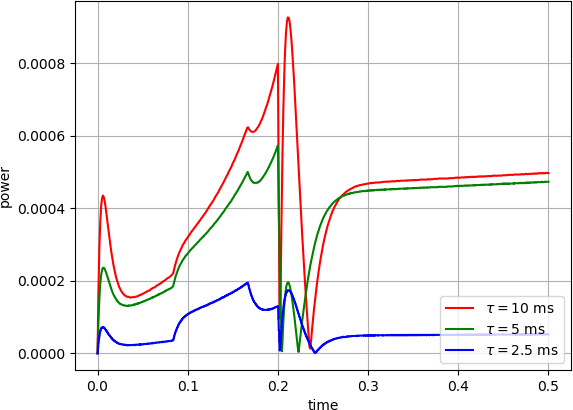
\includegraphics[width=0.8\linewidth]{dif_tau_r_100.png}\\
	\caption{\label{image:canonsummary}Результаты расчета TWIGL-R для различных шагов по времени по диффузионной модели при $\gamma=100$.}
	\label{ris:dif_tau_r_100}
\end{center}
\end{figure}

\begin{figure}[htp]
\begin{center}
	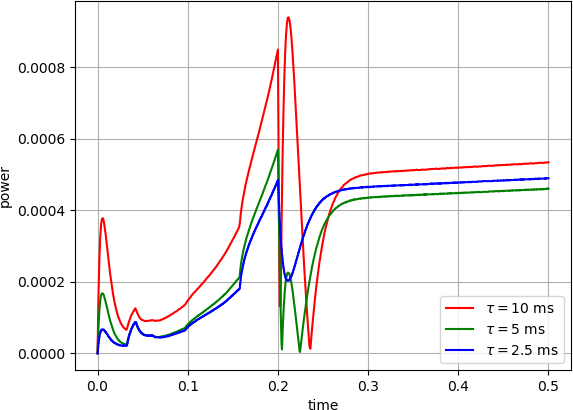
\includegraphics[width=0.8\linewidth]{sp3_tau_r.png}\\
	\caption{\label{image:canonsummary}Результаты расчета TWIGL-R для различных шагов по времени по транспортной sp3 модели.}
	\label{ris:sp3_tau_r}
\end{center}
\end{figure}

\pagebreak
\newpage

\subsubsection{Cценарий №3}
В таблице \ref{table:twigl-c} представлены результаты эталонных решений TWIGL-C при $n=144, p=3, \tau=1$ мс по диффузионной и транспортной моделях.
На рисунке \ref{ris:sp3_ref_c} показано эталонное решение TWIGL-C по транспортной модели, а на рисунке \ref{ris:odds_c} показаны различия диффузионных эталонных решений относительно транспортного эталонного решения. 
Далее, на рисунках \ref{ris:dif_tau_c_0.5}, \ref{ris:dif_tau_c_100}, \ref{ris:sp3_tau_c} показаны отличия при различных шагах по времени относительно эталонных решений.


\begin{table}[htp]
\caption{Различие результатов диффузионного и транспортного расчетов для TWIGL-C.}
\label{table:twigl-c}
\begin{center}
\begin{tabular}{r R{2.5cm} R{2.5cm} R{2.5cm}}
\hline
$t$ & Dif ($\gamma=0.5$) & Dif ($\gamma=100$) & SP$_3$\\
\hline
0.0 & 1.0000 & 1.0000 & 1.0000\\
0.1 & 1.3422  & 1.3393 & 1.3402\\
0.2 & 2.1686  & 2.1580 & 2.1757\\
0.3 & 0.7103  & 0.7119 & 0.7109\\
0.4 & 0.6452 & 0.6470 & 0.6455\\
0.5 & 1.0024  & 1.0024 & 1.0051\\
\hline
\end{tabular}
\end{center}
\end{table}

\begin{figure}[htp]
\begin{center}
	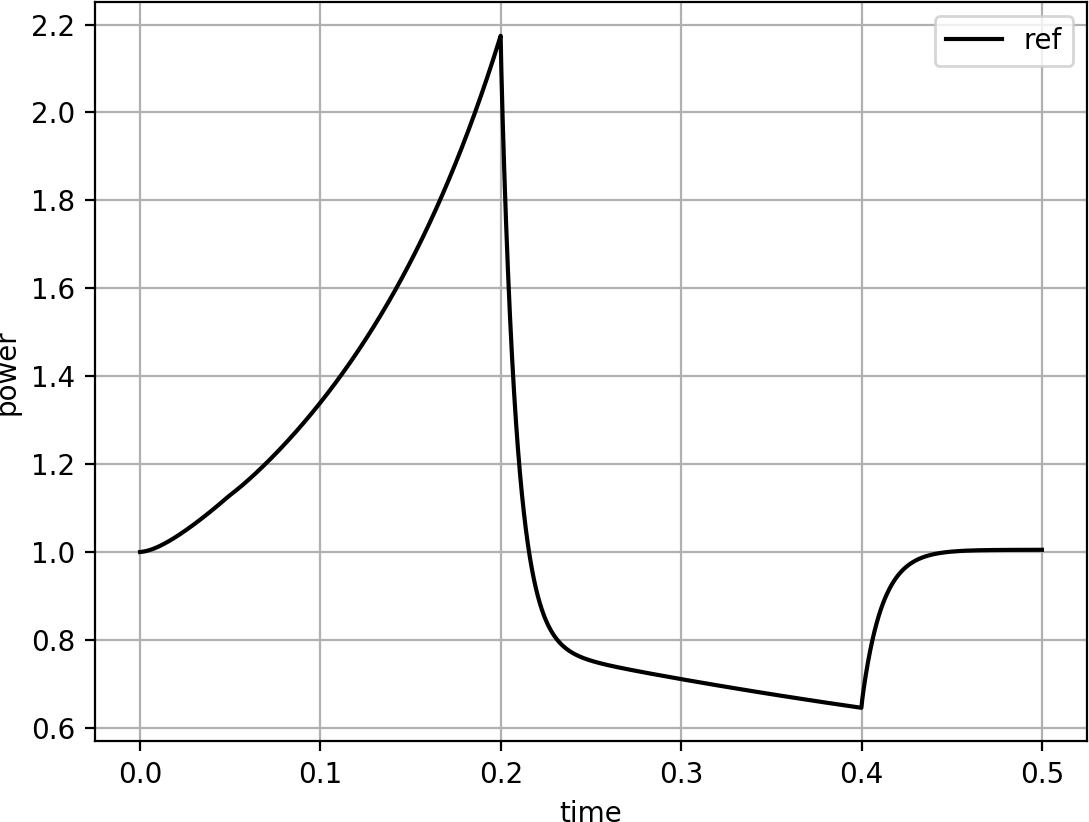
\includegraphics[width=0.8\linewidth]{sp3_ref_c.png}\\
	\caption{\label{image:canonsummary} Эталонное решение TWIGL-C по транспортной SP$_3$ модели.}
	\label{ris:sp3_ref_c}
\end{center}
\end{figure}

\begin{figure}[htp]
\begin{center}
	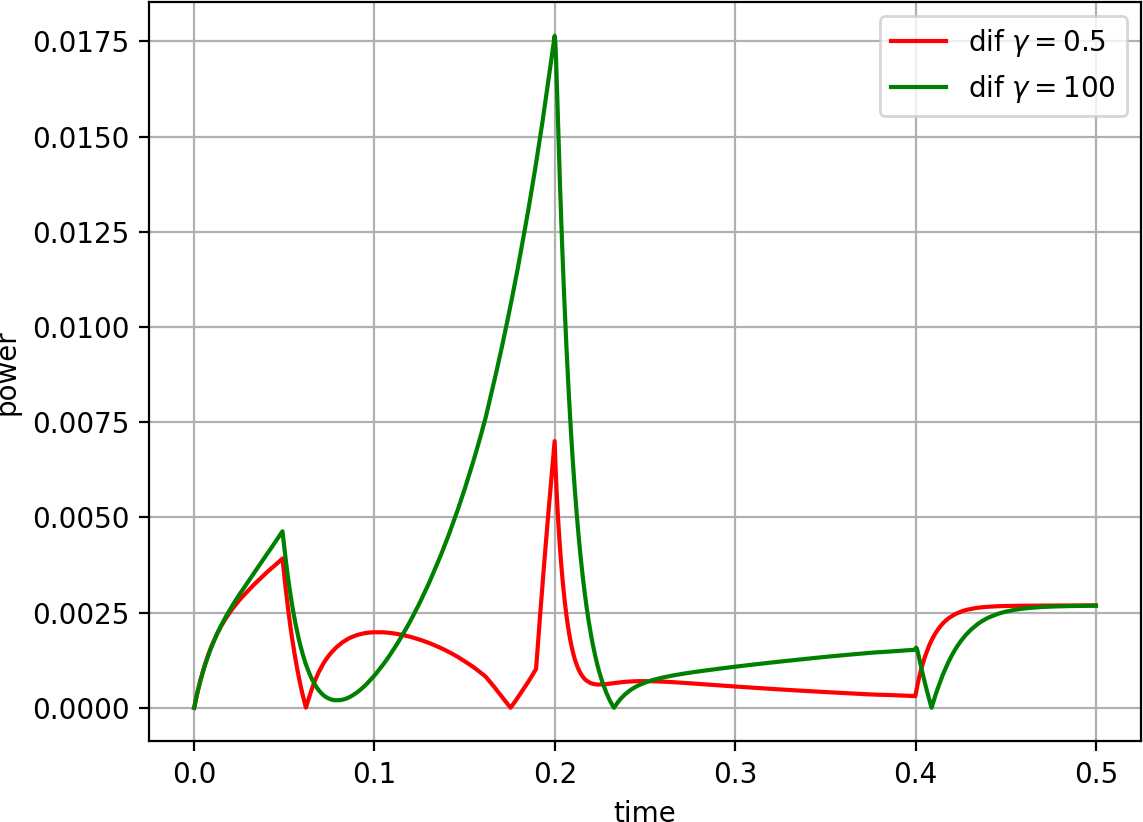
\includegraphics[width=0.8\linewidth]{odds_c.png}\\
	\caption{\label{image:canonsummary} Различия решения TWIGL-C по диффузионной модели от транспортной модели.}
	\label{ris:odds_c}
\end{center}
\end{figure}

\begin{figure}[htp]
\begin{center}
	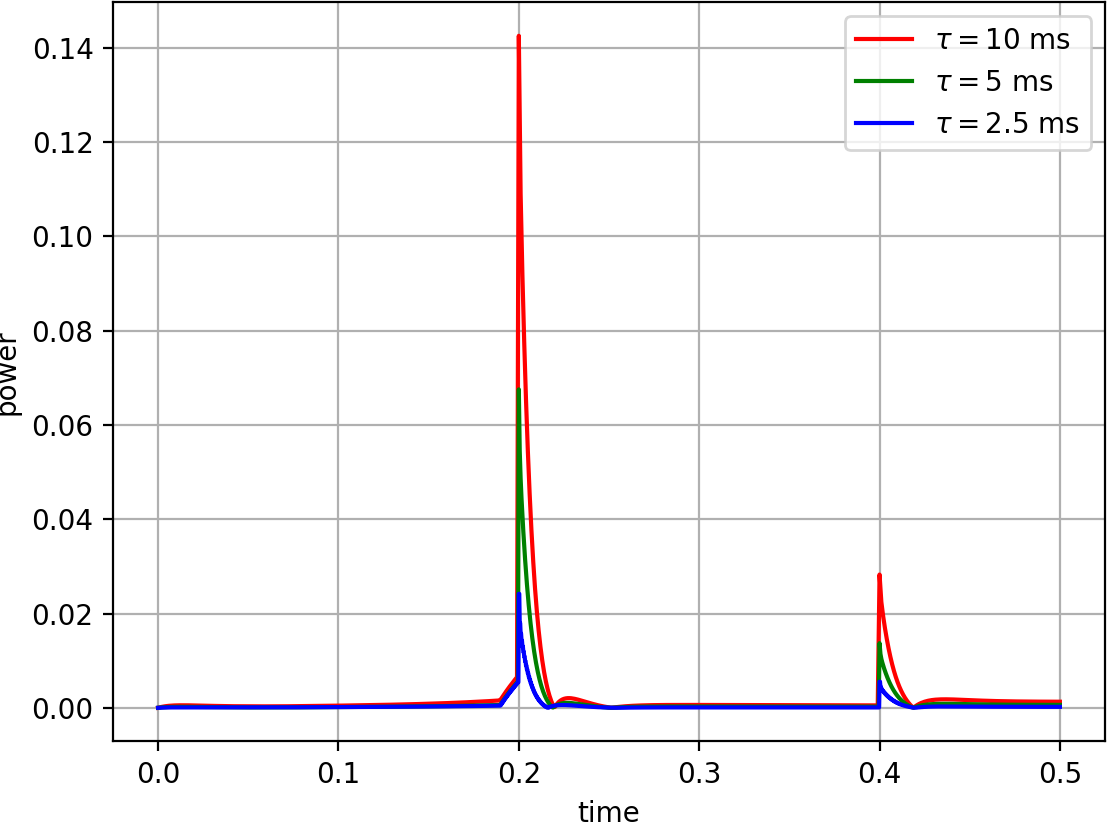
\includegraphics[width=0.8\linewidth]{dif_tau_c.png}\\
	\caption{\label{image:canonsummary}Результаты расчета TWIGL-C для различных шагов по времени по диффузионной модели при $\gamma=0.5$.}
	\label{ris:dif_tau_c_0.5}
\end{center}
\end{figure}

\begin{figure}[htp]
\begin{center}
	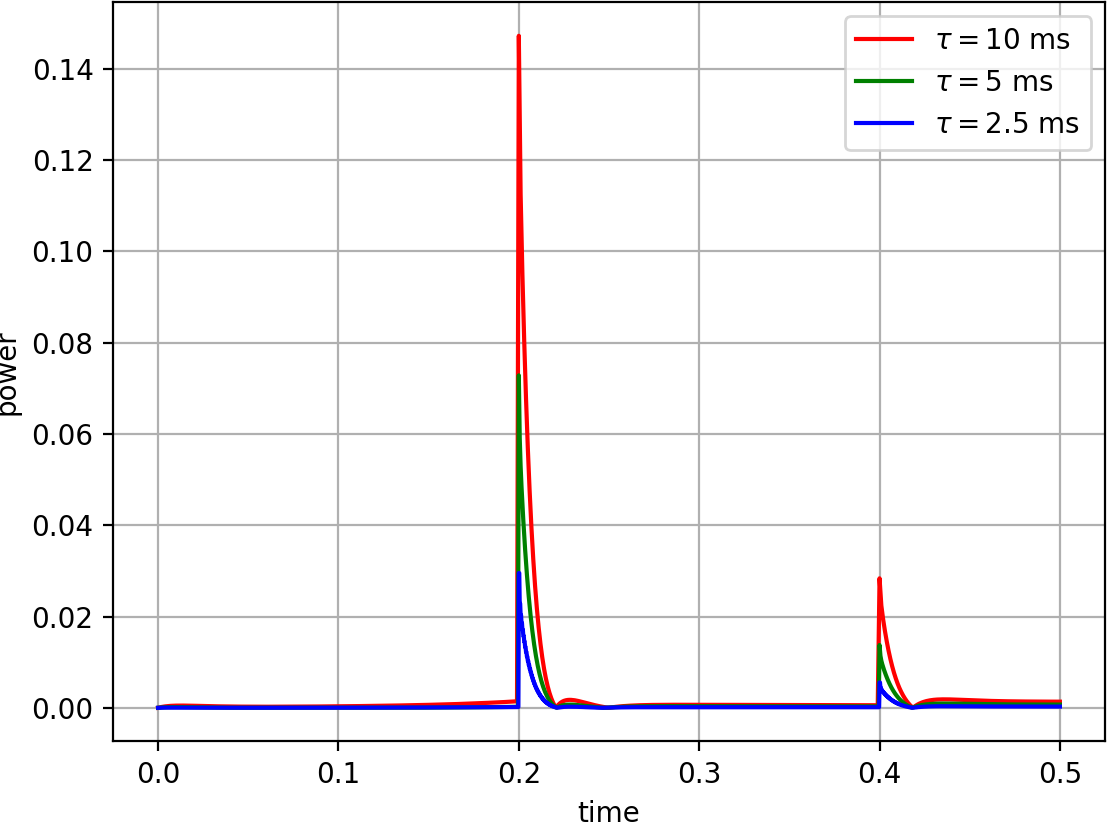
\includegraphics[width=0.8\linewidth]{dif_tau_c_100.png}\\
	\caption{\label{image:canonsummary}Результаты расчета TWIGL-C для различных шагов по времени по диффузионной модели при $\gamma=100$.}
	\label{ris:dif_tau_c_100}
\end{center}
\end{figure}

\begin{figure}[htp]
\begin{center}
	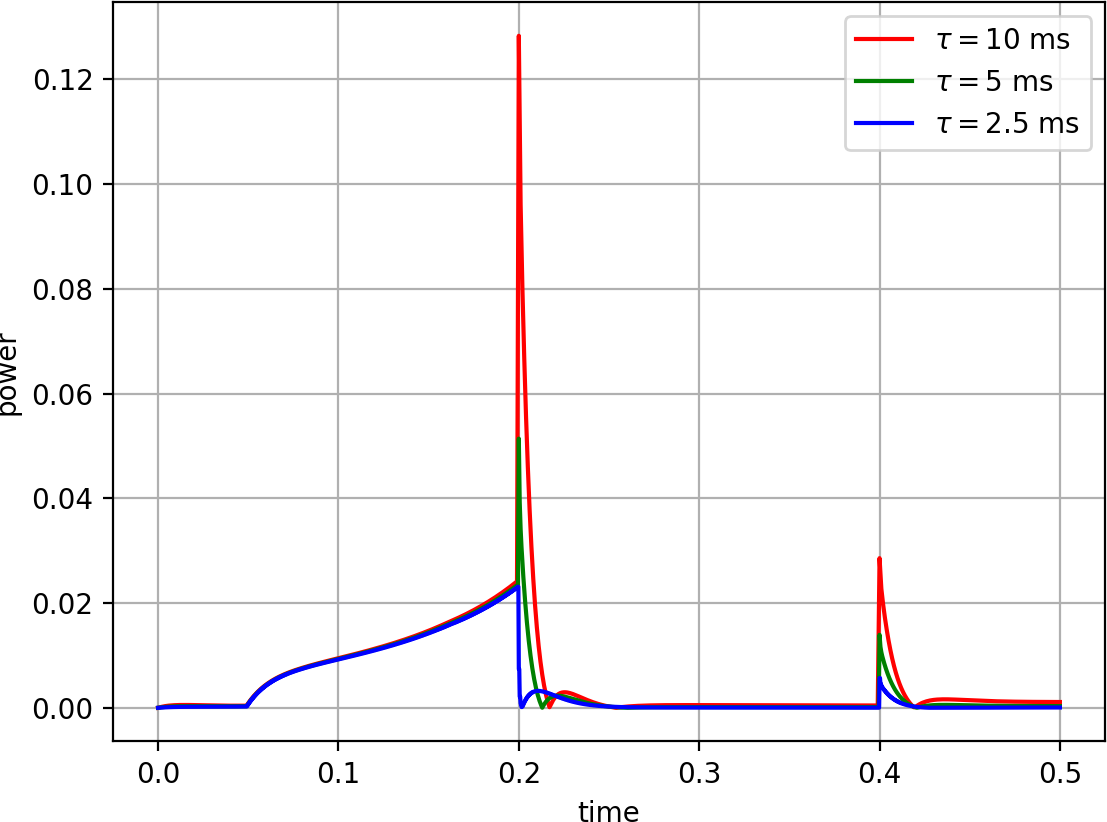
\includegraphics[width=0.8\linewidth]{sp3_tau_c.png}\\
	\caption{\label{image:canonsummary}Результаты расчета TWIGL-C для различных шагов по времени по транспортной sp3 модели.}
	\label{ris:sp3_tau_c}
\end{center}
\end{figure}

% References
%\pagebreak
%\begin{thebibliography}{35}
%
%
%\end{thebibliography}

\end{document}